\chapter{Power conversion}\label{ch:power_conversion}

The full power supply system with the interaction between all of the different regulation stages is shown Figure \ref{fig:circuit_diagram_power}. A half wave rectifier was chosen as the first stage of the power supply system, this was chosen as it requires less diodes than a full wave rectifier, however a drawback is that a larger smoothing capacitor is required. The second part of this power supply system constitutes a SMPS buck converter implemented to decrease the input voltage to an intermediary voltage usable by the final regulation stages. This buck converter works by charging up an inductor, which stores energy in the form of a magnetic field. If the voltage supplied to the inductor is removed it will reverse the polarity of its voltage and will supply the load with the energy stored in its magnetic field. Through this constant switching between the on and off state the converter is able to decrease the voltage from the input to the output at very high efficiency \cite{Gao:2015}.\vspace{4mm} \newline
The \SI{5}{V} regulator was implemented as a linear regulator, which is a device that uses a closed feedback loop to continuously adjust a voltage divider network to maintain a constant output voltage. The main drawback of this regulation topology is that efficiency is limited as the difference between the input and output voltage is dissipated as heat. Finally the \SI{-5}{V} regulator was implemented as a charge pump, which is a type of switching regulator that delivers power by alternatively charging and discharging capacitors and is specifically useful for supplying circuits with a low load current \cite{WebsiteChargePump}.

\begin{figure}[!ht]
  \centering
 \footnotesize
        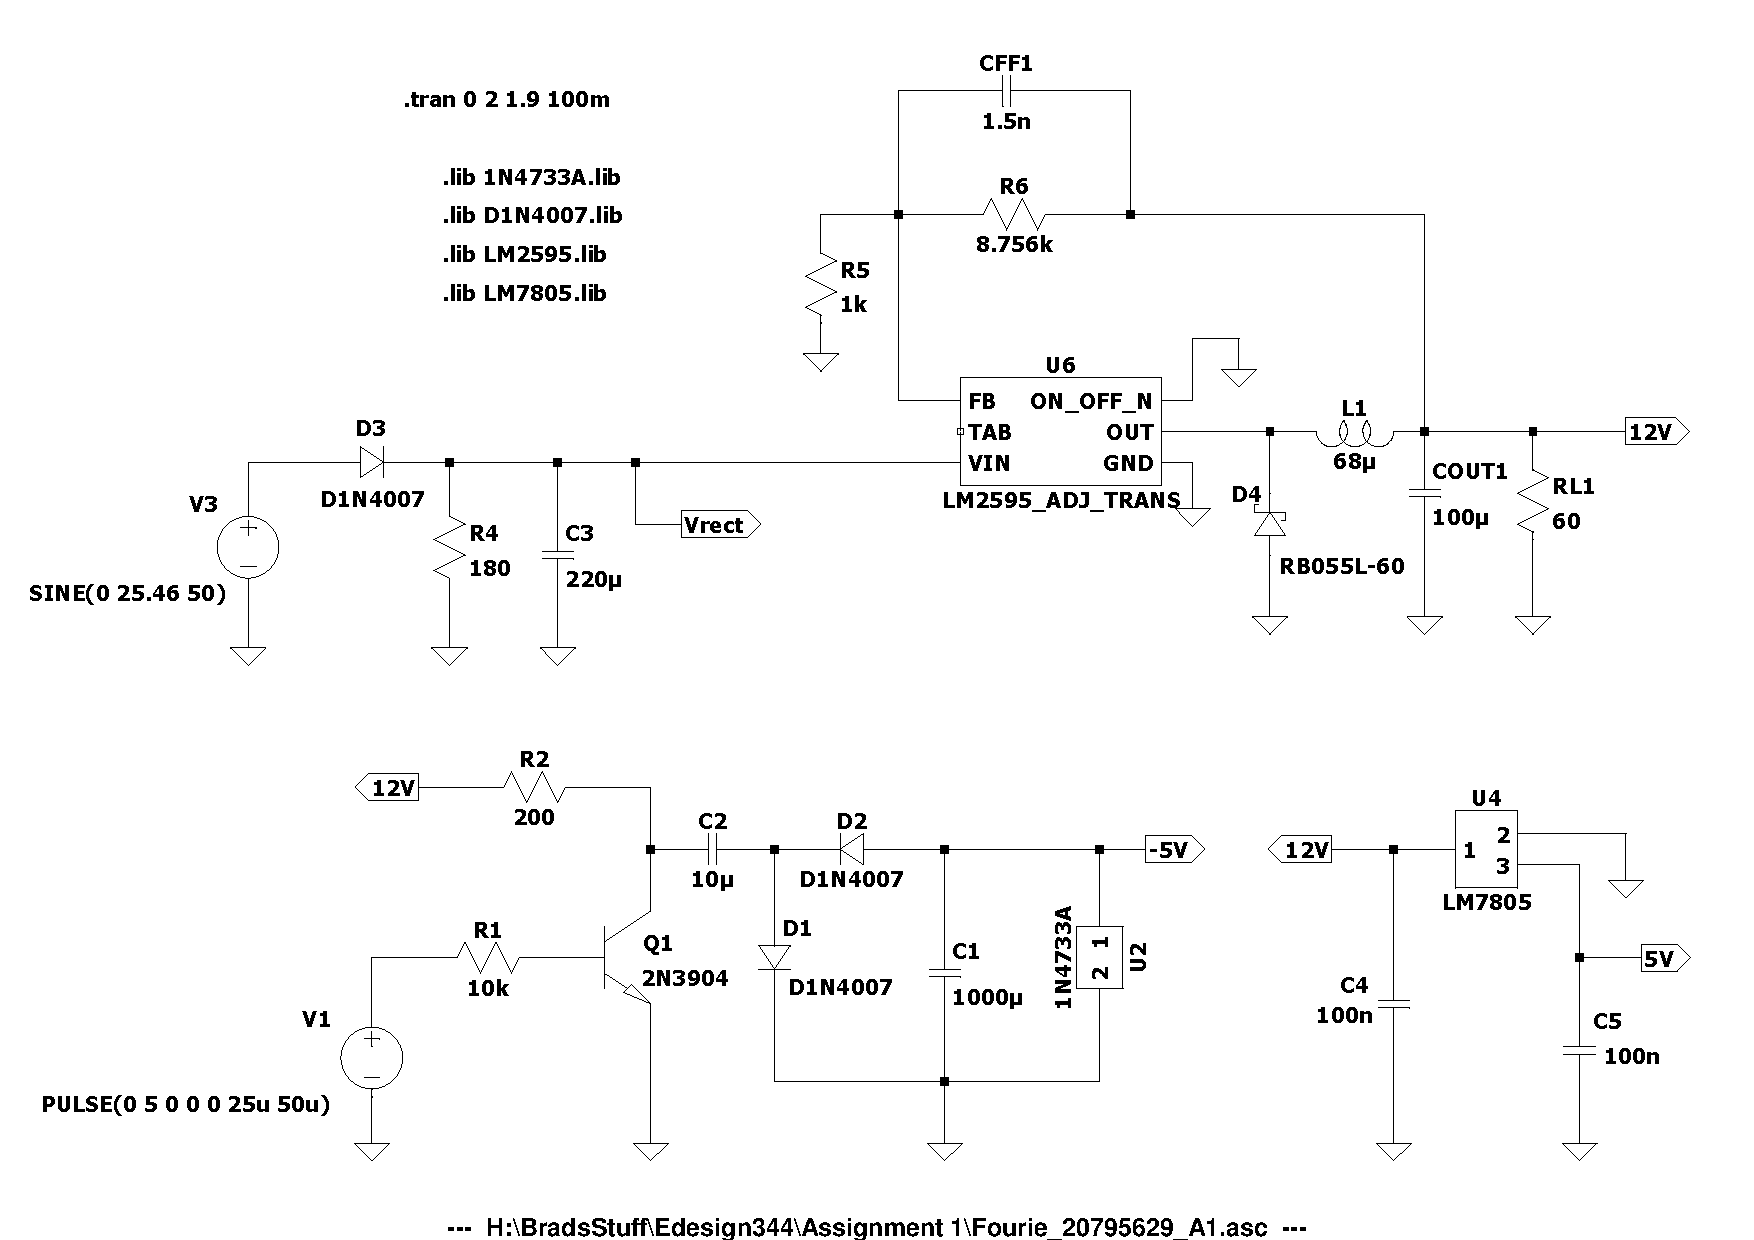
\includegraphics[width=0.75\linewidth]{./Figures/circuit_diagram_power.pdf}
		    \caption{Power conversion circuit diagram.} \label{fig:circuit_diagram_power}
 \end{figure}
%**********************************************
\section{Design} \label{sec:pwr_design}
 
%**********************************************
\subsection{Rectifier}
Firstly a suitable output voltage, allowable output voltage ripple as well as a maximum load requirement had to be chosen. The maximum input voltage was chosen as $\SI{24}{V_{RMS}}$ and a ripple of $50\%$ was chosen, it is worth noting that from \cite{1n4007:2011} the voltage drop over the diode was found as $\SI{1}{V}$ which meant that the output voltage of the rectifier would always be $\SI{1}{V}$ less than the peak value of the sinusoidal input. Referring to the 1N4007 diode datasheet it was confirmed that the full load current draw did not exceed the $\SI{1}{A}$ maximum forward current of the diode. Using Equation \ref{eq:rectifierripple} from \cite{Neaman:2018} the required capacitor was found to be \SI{222.22}{\micro F}, thus a standard \SI{220}{\micro F} was chosen.
\begin{equation}
   V_{r} = \frac{V_{m}}{fRC}
   \label{eq:rectifierripple}. 
\end{equation}

\subsection{Switchmode regulation}
A LM2595 was implemented to control the switching frequency of the switch mode power supply in order to supply an adjustable output of \SI{12}{V}. A series buck regulator in the adjustable output configuration was chosen for the design so that the output could be fine tuned using a potentiometer. The input voltage ranges for the switch mode power supply was chosen as \SI{24.46}{V} to \SI{33.94}{V}, with a maximum supply current chosen as \SI{50}{\milli A}, this was much less than the maximum input voltage of $\SI{45}{V}$ that the regulator is rated for. From the datasheet under these circumstances the regulator operates at roughly $78\%$ efficiency \cite{lm2593:2013}. In order to set the output voltage Equation \ref{eq:smpsresistor} had to be used to choose a ratio of $R_{1}$ to $R_{2}$ to supply the correct output voltage, $R_{1}$ was chosen as $\SI{1}{\kilo \Omega}$, and $V_{ref}$ was given as \SI{1.23}{V}, thus $R_{2}=\SI{8.756}{\kilo \Omega}$. Following this a $\SI{68}{\micro H}$ inductor was chosen following the datasheet. \vspace{4mm} \newline
An output capacitor $C_{out}$ with a low ESR rating, smaller than $\SI{330}{\micro F}$ had to be chosen. A $\SI{100}{\micro F}$ capacitor was chosen, however since this capacitor did not have a low ESR rating a decoupling capacitor had to be placed in parallel with it to remove any ripple voltage due to the high 150kHz switching frequency of the regulator. It is worth noting that this capacitor had to have a voltage rating 1.5 times larger than the 12V output voltage. The same procedure had to be applied for the input bypass capacitor, which was chosen as a $\SI{220}{\micro F}$ capacitor rated for $\SI{50}{V}$ to prevent any large transients from appearing on the input. As an output voltage larger than 10V was chosen for this design a $\SI{1.5}{\nano F}$ ceramic compensation capacitor needed to be added in parallel with $R_{2}$ to provide the necessary stability. Finally a flyback diode $D_1$ had to be added in parallel with the inductor to eliminate any voltage spikes during switching \cite{WebsiteFlyback}. This diode was required to be a fast recovery Schottky diode with a maximum current rating of 1.3 times larger than the load current, and an input voltage 1.25 times larger than the maximum input voltage, for this purpose a 1N5822 was chosen.
\begin{equation}
   V_{out} = V_{ref}(1+\frac{R_{2}}{R_{1}})
   \label{eq:smpsresistor}
\end{equation} 

\subsection{Linear regulation}
A MC78L05 was chosen to supply the $\SI{5}{V}$ rail of the system, since this regulator could handle up to $\SI{35}{V}$ input voltages it was compatible with the maximum $\SI{12}{V}$ output from the intermediary voltage stage. To ensure that the integrated chip could handle the required power requirements the necessary heat sink calculations needed to be completed. \newline 
Given these design requirements a $\SI{7}{V}$ difference was induced across the input and output of the regulator, and a maximum output current of $\SI{40}{\milli A}$ was chosen, which was less than the $\SI{100}{\milli A}$ current the regulator can supply. Furthermore under these conditions a power dissipation of $\SI{280}{\milli W}$ can be expected, which is much less than the $\SI{750}{\milli W}$ maximum power dissipation the regulator is designed for \cite{reg78L05:2002}. By applying Equation \ref{eq:mc78l05temp} from \cite{Perold:2019} and choosing an ambient temperature of $\SI{25}{\degree C}$, the maximum induced temperature was found to be $\SI{67}{\degree C}$, which is far below the maximum allowable operating temperature of $\SI{150}{\degree C}$.\newline
\begin{equation}
   T_{max} = P_{max}(R_{\Theta _{JA}}) + T_{A}
   \label{eq:mc78l05temp}
\end{equation}
An additional capacitor was added to the input of the regulator as to reject attenuation and specifically AC noise from the switchmode regulator. Another capacitor was added to the output of the regulator in order to improve stability and to improve the regulators transient response, both of these capacitors were chosen according to datasheet recommendations.

\subsection{Charge pump regulation}
The first step in designing the charge pump was to select a charge tank capacitor that would ensure a continuous supply of current to the load. For the purpose of this design a $\SI{1}{\milli F}$ capacitor was chosen to supply a maximum of 5mA, and to remove any ripple voltages a $\SI{10}{\nano F}$ capacitor was placed in parallel with it. A secondary smaller capacitor had to be designed to discharge completely within the period of the $\SI{10}{\kilo Hz}$ pulse train to supply charge to the larger capacitor, here a low ESR $\SI{10}{\micro F}$ capacitor was chosen.\vspace{4mm} \newline
A common emitter configuration was chosen to provide a current gain to the output whilst providing no voltage gain, with suitable collector and base resistors designed such that the transistor could turn on and current could flow such as to charge up the capacitor. A base resistor of $\SI{10}{\kilo \Omega}$ was chosen to minimize current losses through the transistor, and a collector resistor of $\SI{200}{\Omega}$ was chosen to supply enough current to the $\SI{-5}{V}$ rail without exceeding the $\SI{625}{\milli W}$ maximum power rating of the transistor.

%**********************************************
\section{Simulation} \label{sec:pwr_simu}
%**********************************************
The rectifier circuit was simulated with a $\SI{18}{V_{RMS}}$ input, with this maximum voltage ripple shown in Figure \ref{subfig:pwr_simu_rect}. For this nominal supply input a ripple of only $34.8\%$ was reported, which was below the maximum ripple designed for. The complete power regulation system was simulated as to obtain the steady state DC voltage values of the rails, Figure \ref{subfig:pwr_simu_rails_pos} displays the output of the $\SI{5}{V}$ regulator and Figure \ref{subfig:pwr_simu_rails_neg} displays the output of the $\SI{-5}{V}$ regulator, from this we can confirm that by simulation the power supply system was designed correctly.

%**********************************************
\section{Measurements} \label{sec:pwr_meas}
%**********************************************
The power system as a whole was tested with the rail voltages supplied by the charge pump and linear regulators respectively, which in turn were powered by the intermediary voltage stage which received its input from the rectified transformer output. The measured output voltage of the linear regulator was found to be $\SI{5.12}{V}$ under full load conditions supplying $\SI{40}{\milli A}$ as shown in Figure \ref{subfig:pwr_meas_rails_pos}, under these circumstances the efficiency of the regulator was calculated as $37.3\%$ using Equation \ref{eq:efficiency} at a maximum quiescent current of $\SI{5.5}{\milli A}$. As can be seen in Figure \ref{subfig:pwr_meas_noise_pos} a noise level of less than $\SI{10}{\milli V}$ peak to peak was measured on the $\SI{5}{V}$ rail, which confirms that the regulator met all the required specifications.
\begin{equation}
   \eta = \frac{P_{out}}{P_{in}}
   \label{eq:efficiency}
\end{equation}
The charge pump supplied a stable $\SI{-5.12}{V}$ output under no load conditions as can be seen in Figure \ref{subfig:pwr_meas_rails_neg}, with noise not exceeding $\SI{9.28}{\milli V}$ peak to peak as can be seen in Sub figure \ref{subfig:pwr_meas_noise_neg}. After a $\SI{10}{\kilo \Omega}$ load was applied to regulator, it was found that the output voltage level dropped to $\SI{-4.76}{V}$.

\section{Summary and implementation}
The power regulation system implemented for this system met all of the design requirements and can be seen in Figure \ref{subfig:pwr_pcb}. The rectification stage of the power supply which rectified the transformer supply voltage had a ripple voltage of less than 35\%, and could successfully supply the input voltage and current required for the intermediary switchmode power supply stage. This buck converter output a stable $\SI{12}{V}$ output and successfully supplied the inputs to both the charge pump and linear regulator. The linear regulator supplying the $\SI{5}{V}$ rail operated successfully under full load conditions and could supply a steady output under all required loading conditions, however the charge pump supplying the $\SI{-5}{V}$ rail could not supply enough current for the purpose of this design, therefore it was decided that it would not be used to supply the signal conditioning circuitry.

\begin{figure}[!ht]
    \centering
  	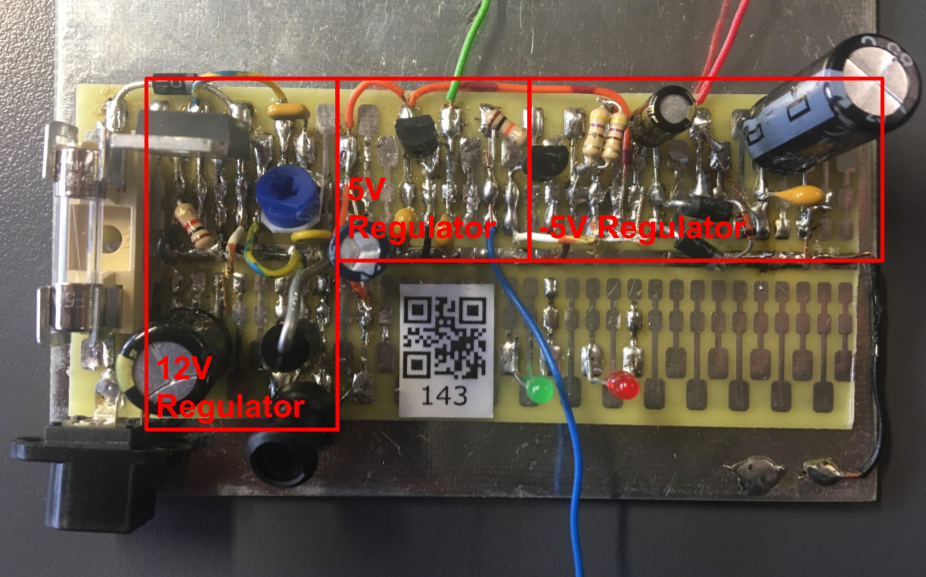
\includegraphics[width=0.5\linewidth]{./Figures/pwr_pcb.png}
	\caption{Implementation of the power conversion circuitry. } \label{subfig:pwr_pcb}
\end{figure}

\begin{figure}
 \footnotesize
 \centering
    \begin{subfigure}[]{0.35\textwidth}
              \centering
  		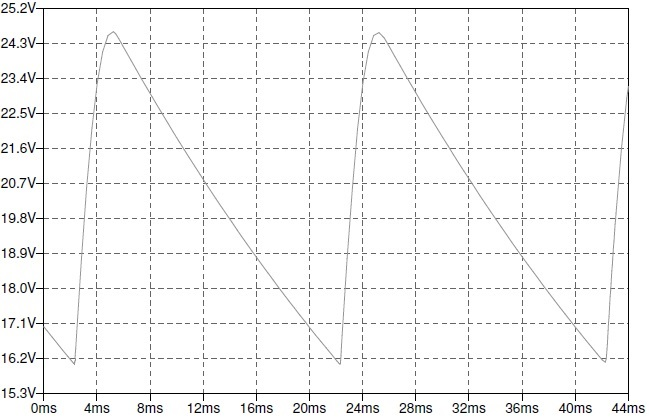
\includegraphics[width=1\linewidth]{./Figures/pwr_simu_rect.JPG}
		    \caption{} \label{subfig:pwr_simu_rect}
     \end{subfigure}
          \begin{subfigure}[]{0.35\textwidth}
             \centering
  		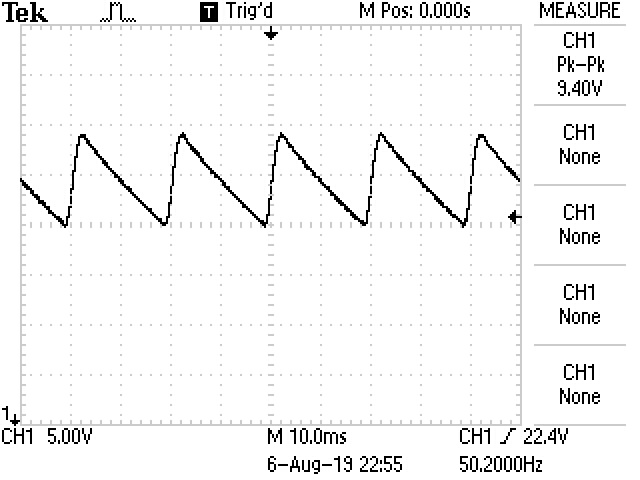
\includegraphics[width=1.0\linewidth]{./Figures/pwr_meas_rect.jpg}
		   \caption{ } \label{subfig:pwr_meas_rect}
     \end{subfigure}
    \begin{subfigure}[]{0.35\textwidth}
              \centering
  		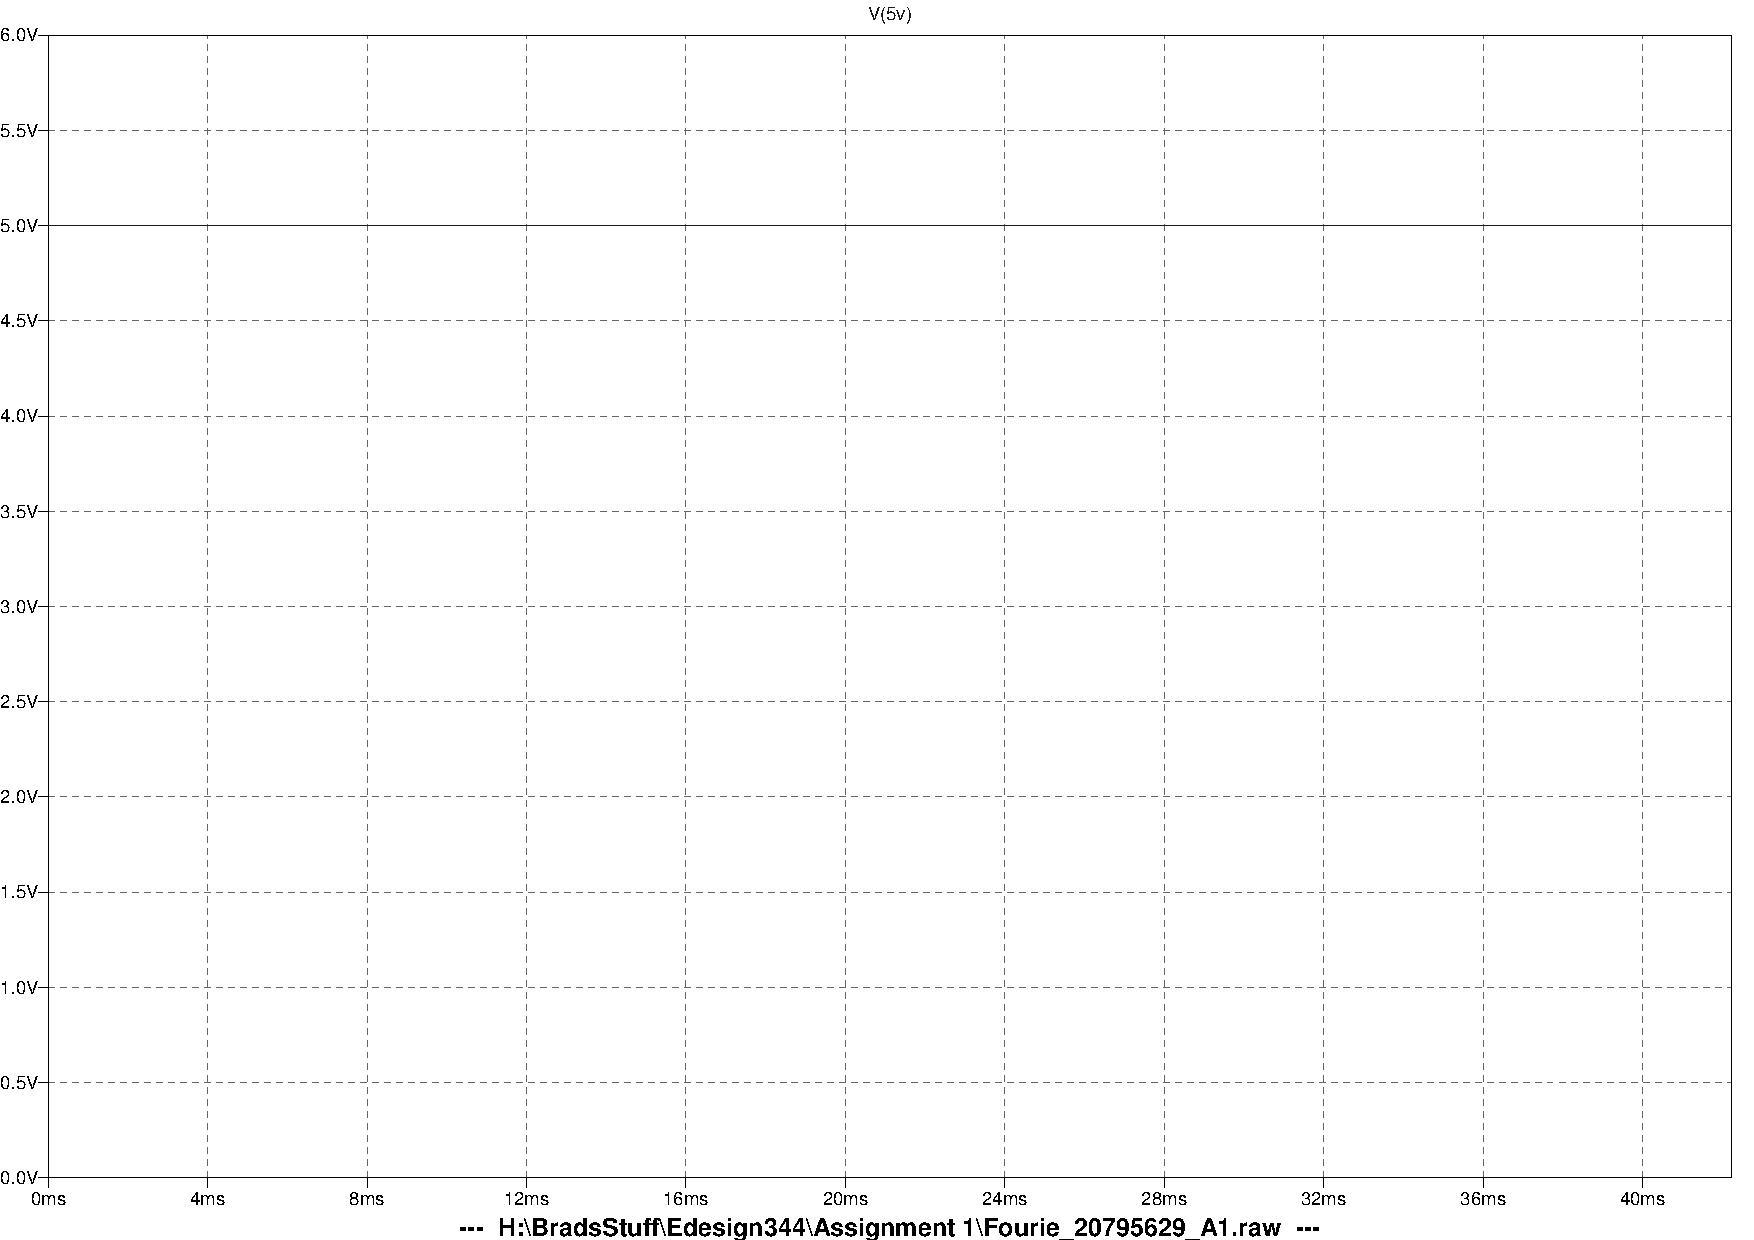
\includegraphics[width=1\linewidth]{./Figures/pwr_simu_rails_pos.pdf}
		    \caption{} \label{subfig:pwr_simu_rails_pos}
     \end{subfigure}
    \begin{subfigure}[]{0.35\textwidth}
              \centering
  		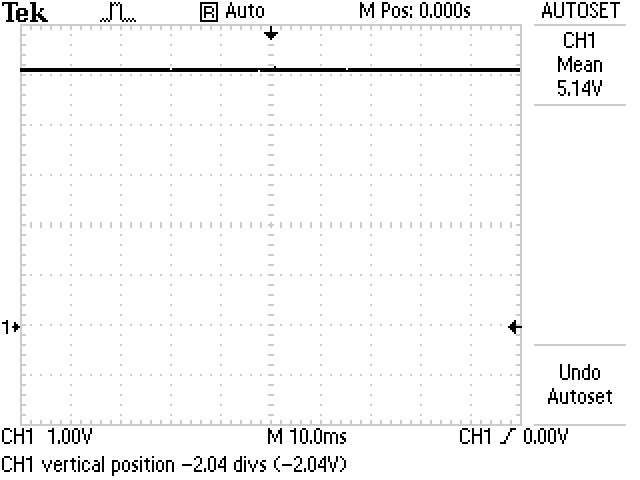
\includegraphics[width=1\linewidth]{./Figures/pwr_meas_rails_pos.JPG}
		    \caption{} \label{subfig:pwr_meas_rails_pos}
     \end{subfigure}
    \begin{subfigure}[]{0.35\textwidth}
             \centering
      		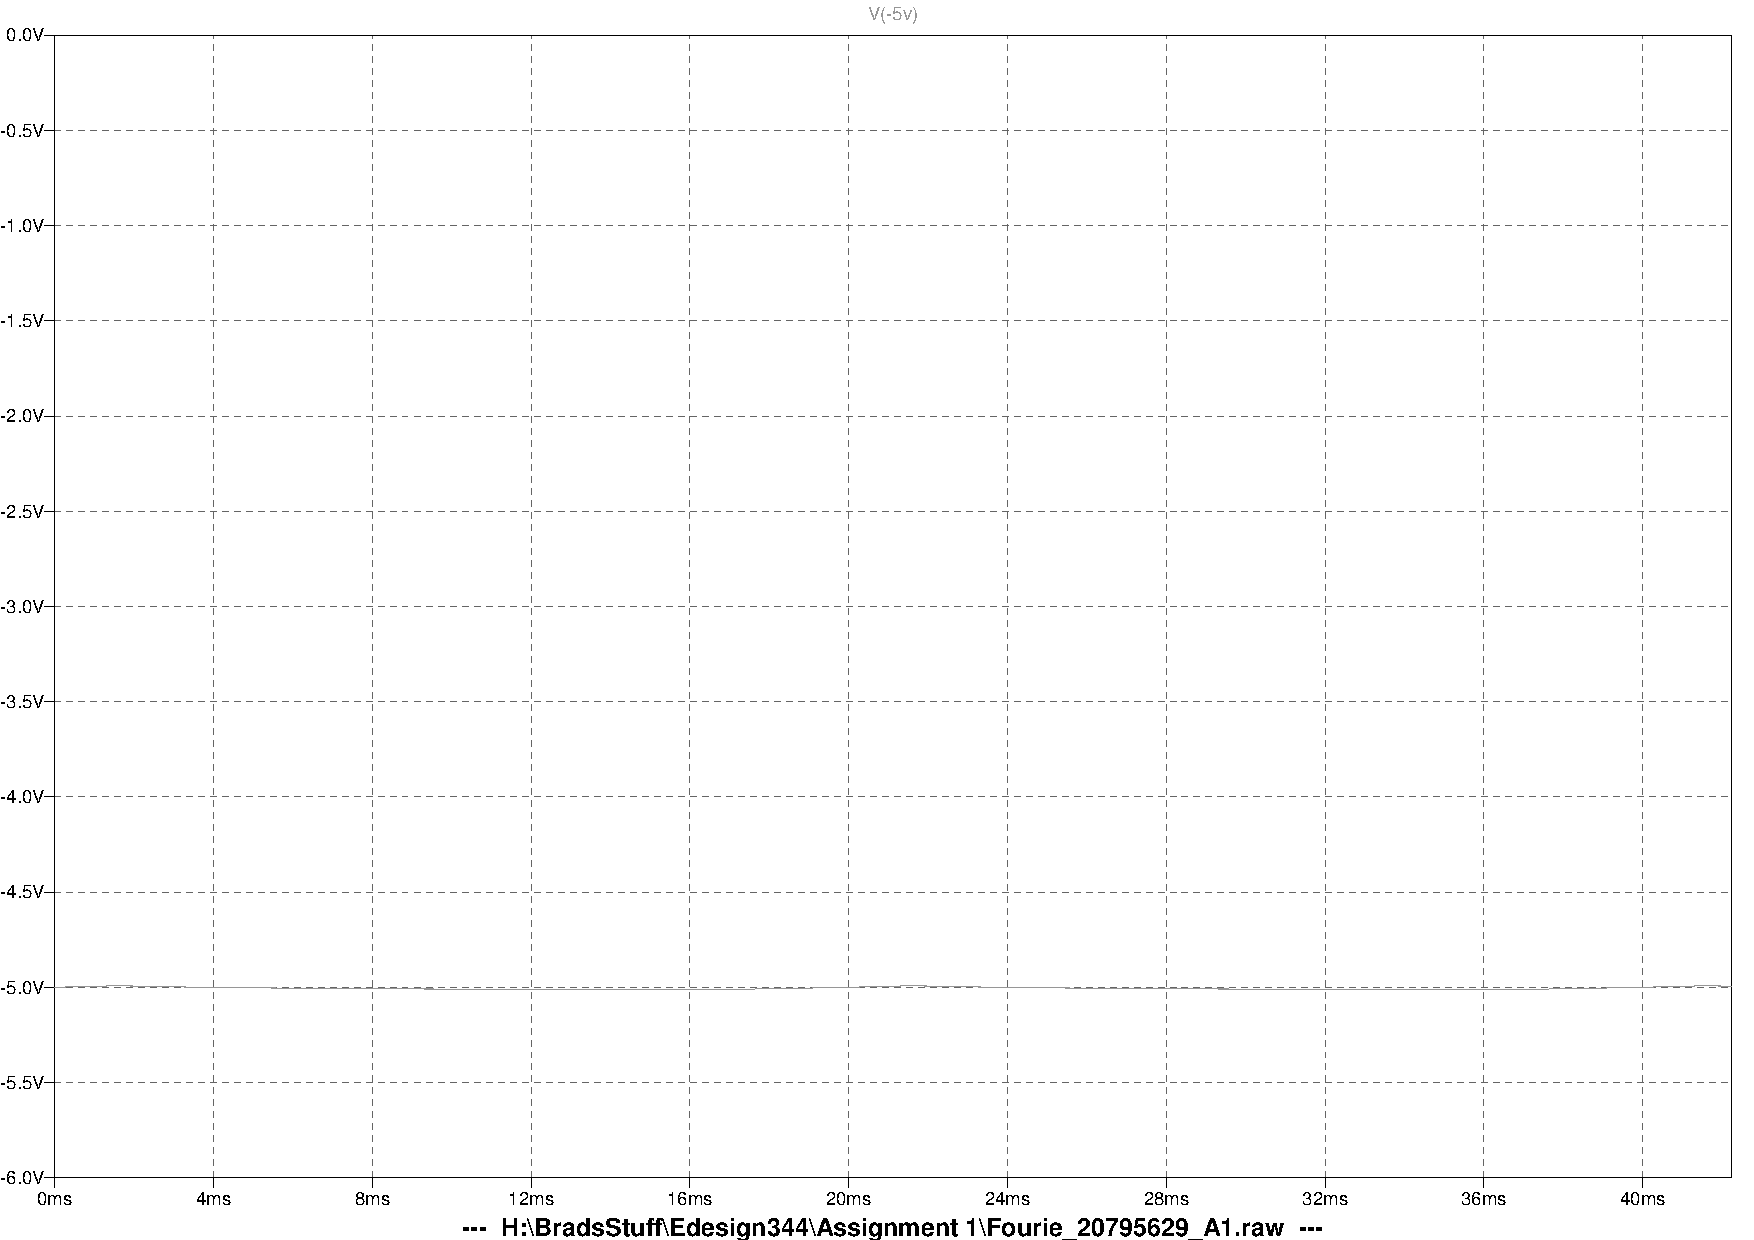
\includegraphics[width=1.0\linewidth]{./Figures/pwr_simu_rails_neg.pdf}
		   \caption{ } \label{subfig:pwr_simu_rails_neg}
     \end{subfigure}
    \begin{subfigure}[]{0.35\textwidth}
             \centering
  		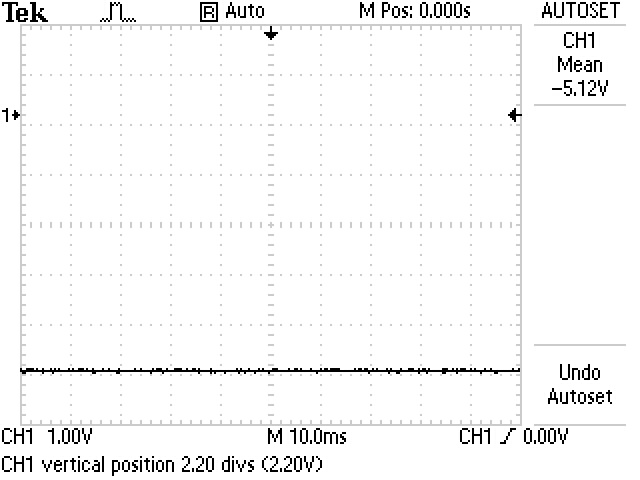
\includegraphics[width=1.0\linewidth]{./Figures/pwr_meas_rails_neg.JPG}
		   \caption{ } \label{subfig:pwr_meas_rails_neg}
     \end{subfigure}
    \begin{subfigure}[]{0.35\textwidth}
              \centering
  		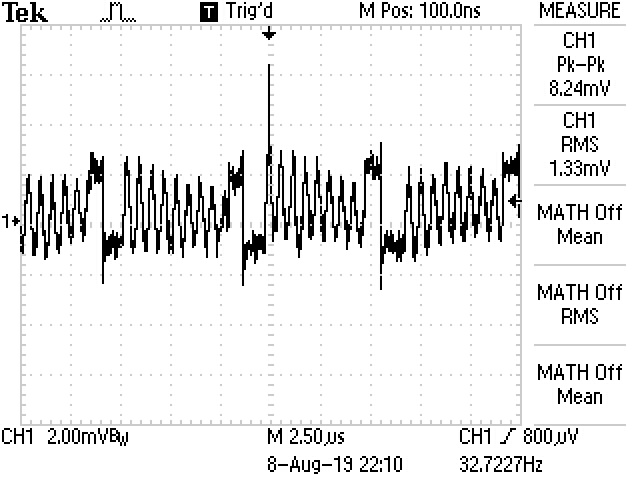
\includegraphics[width=1\linewidth]{./Figures/pwr_meas_noise_pos.JPG}
		    \caption{} \label{subfig:pwr_meas_noise_pos}
     \end{subfigure}
    \begin{subfigure}[]{0.35\textwidth}
             \centering
  		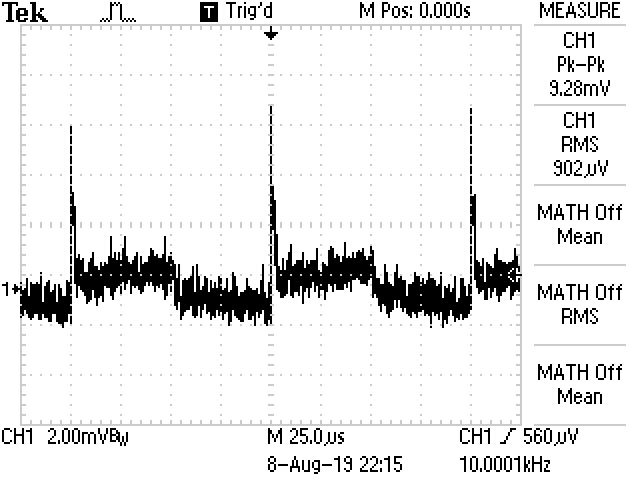
\includegraphics[width=1.0\linewidth]{./Figures/pwr_meas_noise_neg.JPG}
		   \caption{ } \label{subfig:pwr_meas_noise_neg}
     \end{subfigure}
   \caption[Measured regulated output voltage plots]{Power conditioning: (a) Simulation of the rectification showing the rectified signal. (b)  Measurement of the rectification showing the rectified signal.  (c)  Simulation output of the positive voltage rail level. (d) Measurement of the positive voltage rail level. (e)  Simulation output of the negative voltage rail level. (g) Measurement of the negative voltage rail level. (g)  Measurement of the noise on the postive voltage rail. (h) Measurement of the noise on the negative voltage rail. }
    \label{fig:simulation_results_box}
 \end{figure}

